



\section{Financial Markets and the Study of War}
\label{bonds_battles:sec:barg-theory-war}

Financial markets are useful in the study of war in several ways.
First, they provide a measure of the the costs of war \parencites{SchneiderTroeger2006}{GuidolinLaFerrara2010}.
Second, financial markets themselves are a key actor or mechanism in several theories of war, such as the ``Capitalist Peace'' \parencites{Gartzke2007}{DafoeKelsey2014a}, in which markets signal the costs of war, or \textcite{Slantchev2012a} in which debt financing creates a commitment problem.
Third, in some cases, the prices of financial assets act like a prediction market of the expected onset or outcome of war, and be used to assess theories of war initiation and termination.%
\footnote{See Chapter \ref{cha:financ-mark-onset} for an analysis of how financial markets assessed the probability of the onset of the American Civil War.}
In this paper, I focus on the third case, and use the yields of U.S. government bonds to measure expectations of the outcome of the American Civil War.%
\footnote{I will use the term ``outcome'' to mean the duration, cost, and victor of the war. I will use the term ``result'' to the outcomes: ``Union victory'' or ``Confederate victory''.}


\subsection{How the Prices of Financial Assets Relate to War Outcomes}
\label{bonds_battles:sec:how-prices-financial}

At its most basic level, a financial asset is a claim on a stream of future, possibly uncertain, cash flows.%
\footnote{
  This discussion largely follows the discussion in \textcite[673]{GuidolinLaFerrara2010}; refer to them for more detail.
  See also \textcite{HaberMitchenerOosterlinckEtAl2015}.
  See any introductory finance textbook or course notes for more information.
  See \textcite{Chan-Lau2006} for an overview of market-based measures of sovereign risk.
}
For example, a coupon bond pays a set number of coupons at specified times and its face value on maturity, and a stock pays out dividends.
Both because these cash flows are in the future and because their payment may be uncertain, these cash flows are discounted.
And the current price of a financial asset is the value of those discounted cash flows.
Slightly more formally, the current price ($P_{t}$) of a financial asset is
\begin{equation}
  \label{bonds_battles:eq:3}
  P_{t} = \sum{j = 1}^{H} \frac{\E_{t + j}\left(C_{t + j} | \mathcal{I}_{t}\right)}{1 + \E_{t}\left(\delta_{t+j} | \mathcal{I}_{t}\right)}
\end{equation}
where $H$ is the number of cash flows, $C_{t + j}$ is the cash flow at time $t + j$, and $\delta_{t + j}$ is the discount rate for time $t + j$, and $\mathcal{I}_{t}$ is the information available to the market at the current time $t$.
The discount rate often consist of a risk free rate and some premium specific to asset, both of which may be time-varying.
Riskiness of the asset can also be incorporated in $\E(C_{t}| \mathcal{I}_{t})$ if the expectation incorporates some probability of default.
The key feature of Equation (\ref{bonds_battles:eq:3}) is that since all of the inputs of the price are in the expectations of the future conditioned on current information.
Thus events can change the price so much as so much as they update the expectations of the market about future cash flows and future risk premia.

Since the prices of financial assets are a function of expectations about future cash flows and risk premia, assets in which the those future cash flows or risk premium are largely contingent on some outcome of a war are a proxy of expectations about that war outcome.
The ideal asset would be a binary option, which pays out a non-zero amount if the war outcome of interest occurs and zero otherwise.
Then, with assumptions about the risk-preferences of the market, the probability of the war outcome can be easily extracted from the price.
Binary options are often associated with prediction markets, there are several examples of prediction markets of political events. 
The Iowa Electronic Market for U.S. presidential elections.%
\footnote{
  See \textcite{WolfersZitzewitz2004} for an overview of prediction markets.
  \textcite{RhodeStrumpf2004a} discusses historical betting markets on U.S. presidential elections in the late nineteenth-early twentieth century, which unfortunately for me were not formalized until 1884.
}
Other examples include contracts by Intrade and Tradesports which in addition to presidential elections, offered contracts for when Saddam Hussein would be removed as the president of Iraq, when Osama Bin Laden would be either killed or captured, and when a there would be a U.S. or Israeli airstrike against Iran.%
\footnote{
  The Saddam contract issued by Tradesports is used in \textcite{LeighWolfersEtAl2003}.
  See \url{http://intrade-archive.appspot.com/event.jsp?event=4272}, \url{http://intrade-archive.appspot.com/event.jsp?event=37985} for the Intrade contracts.
}
Unfortunately for the researcher, these prediction markets in political events are not widespread in the present, and not available historically for wars.
However, financial assets in which the cash flows or risk premia are contingent on a war outcome are effectively prediction markets for that war outcome.%
\footnote{
  Although it may not always be the war outcome that the researcher is most interested in.
  Even if it is clear that the asset is a function of the war outcome, it may not be transparent to the researcher exactly what outcome(s) the asset is a function of.
}
One asset in particular is likely to be highly sensitive to war outcomes: sovereign bonds issued by the belligerents.
In general, the sovereign bonds issued by belligerents is sensitive will be sensitive to two aspects of the war outcome.
First, the riskiness of a belligerent's sovereign bond is a function of the expected cost of the war.
Wars are costly and wars are generally paid by debt \parencite{Slantchev2012a}.
A more costly war almost directly implies a higher debt burden and either higher risk premia or a higher probability of default for the bond (lower price).
This cost is also more than just the expenditures of the government. 
The destruction of human capital (military and civilian casualties) and physical capital has influences on the expected economic growth of that country, and thus its future resources with which to pay off the debt.
These expectations of cost incorporate both expectations about the intensity of the war, and expectations about its duration.
Second, the riskiness of a belligerent's sovereign bond is a function of whether the belligerent is expected to win or lose the war.
Victory in war can mean more territory and greater resources to pay off debt; a loss can mean the converse.
In some cases, especially rebel sides in civil wars, a defeat can mean a loss of sovereignty and a default on their debt, as was the case with the Confederate States.%
\footnote{See One of the clauses of the Fourteenth Amendment of the constitution makes this repudiation explicit.}
More generally, losing states may tend to default on their debt with a higher probability \parencite{Slantchev2012a}.
In general, the price of a bond is some weighted function of all of these expectations about what the outcome of the war will be and how those outcomes will effect the ability of the belligerent to repay.
For some bonds, it may even be possible to back out the probability of a specific outcome.
\textcite{HaberMitchenerOosterlinckEtAl2015} focus on cases in which rebels issued bonds in civil wars (American Civil War, Chinese Civil War, and the Spanish Civil War) and estimate the probability that the rebel side will win.
Another method is by using the prices of several assets from different sides, it may also be possible estimate expectations of victory and defeat; see \textcite{Hall2004} and \textcite{McCandless1996}.
However, in general, it may not be possible to disentangle expectations about the cost and outcomes of the war for the belligerents. 
And that is not necessarily a bad thing.
By putting all outcomes on the same scale, their effect on the long run fiscal outlook of the belligerent, the prices of sovereign bonds are able to provide a single, if incomplete, measure of the war outcome for each belligerent that incorporates both the costs and benefits of the war.
Because interest rates are expectations and are generally available at a high frequency, they provide a measure of real-time expectations about the war.
Sovereign bonds are not the only financial assets which could be used as a proxy for war outcomes, stock market indices or specific sectors thereof \textcites{ChenSiems2004}{SchneiderTroeger2006}{WolfersZitzewitz2009}, exchange rates \textcites{Hall2004}, and commodities \textcites{WolfersZitzewitz2009}, respond to conflict in some cases and may be able to be used as proxies for expectations about war outcomes.
However, The specifics of how different assets relate to expected war outcomes is not universal, and in each case the researcher should think through how the specific financial asset relates to the war outcome of interest.%
when using the price of a financial asset as a proxy for an expected war outcome, it is also necessary that its price is primarily influenced by that war outcome and not other factors.
For example, when studying the Iraq War, it would be implausible to use the interest rates of U.S. Treasury bonds or the S\&P 500 index since the effect of the war one way or another is likely a small influence on them.%
\footnote{
  It is still possible to ask questions such as how much influence did events related to the Iraq War have on the stock market, as in \text{WolfersZitzewitz2009}.
  It would just be difficult to ask the inverse question which may be of more interest to political science research; given that the stock market is proxying expectations of the Iraq War, what events had the largest influence on it.
 }
But it is plausible to use bonds issued by Iraq, if they had issued in 2003, because the war outcome plausibly would be the most important factor influencing them.
This is not out of concern of confounding variable and factors that are not correlated with the war outcome can be a problem.
The concern is that the signal (war outcome) to noise (other factors that cannot be controlled for) ratio of the price is high enough that it is plausible to use the price as a proxy for the war outcome.
One shortcoming of the use of the sovereign bonds, or most financial assets, as proxies for expectations of war outcomes is that they will only be able to proxy for war outcomes so long as those outcomes has some influence on either cash flows or risk premia. 
Some policy objectives of a war, \eg{}national pride or the abolition of slavery in the American Civil War, may be important to the belligerents and of interest to the researcher, but if they do not affect future cash flows or risk premia, then the prices of financial assets have little to say about them.

In this paper, instead of prices, I use the yields to maturity of coupon bonds. 
The yield to maturity of a coupon bond can be found by taking a known price and cash flow schedule in Equation (\ref{bonds_battles:eq:3}) as solving for a single discount rate.
For example, assuming continuous compounding for simplicity, the yield to maturity, $y$, of a bond is the solution to
\begin{equation}
  \label{bonds_battles:eq:5}
  P_{t} = \sum_{j = 1}^{H} C_{t + j} e^{-y j} \text{.}
\end{equation}
The interest rate moves inversely to the price: a higher yield corresponds to a lower price, and vice-versa.
The riskier a bond is, the lower the price and the higher the yield.
%I use the yield to maturity of the bonds rather than their prices,  because prices deterministically drift towards par with time and because they are more interpretable.
% interpretation of risk in terms of default




\subsection{How the Financial Markets Can Improve Our Understanding of War}
\label{bonds_battles:sec:how-prices-financial-1}

Since \parencite{Fearon1995}, the bargaining theory of war has been the dominant theory of war \parencite{Reiter2003}.%
\footnote{See CITES.}
Since \textcite{Fearon1995}, a series of papers developed the theory of how fighting and bargaining interact within war \parencites{FilsonWerner2002}{Slantchev2003}{SmithStam2004}{Powell2004}{LeventogluSlantchev2007}{LangloisLanglois2009}{WolfordReiterCarrubba2011}.
While there has been extensive work in modeling this war (CITES), the the core mechanisms of the theory has not been amenable to empirical, and especially quantitative, analysis.
The prices of financial assets can improve our understanding of theories of war in two ways: expanding the number of cases in which the analysis can be performed, and providing a measure of surprising events.

A primary reason for this for this relative absence of work is the difficulty of obtaining the necessary data to evaluate the implications of the bargaining theory of war.
While the secondary implications of the bargaining theory of war have been tested, the direct implications and the mechanisms of the theory require data on the belligerents' estimates of capabilities and resolve, and bargaining offers \parencite[32]{Reiter2003}.
Due to the lack of detailed data for many wars as well as concerns about the comparability of wars, using within case analysis is an appealing methodology for analyzing the effect of conflict on war termination.
Financial market data provides a measure related to a political science outcome of interest, the war termination, that varies within war.

Among these, data on intra-war combat events, namely battles, would appear to be the most readily available.
Yet, the existing data on battles is generally both poor quality and quantity.
As of yet, there exists no battle-level equivalent with the comprehensive datasets such as the Correlates of War \parencite{SarkeesWayman2010} or the Uppsala Conflict Data Program.
The only existing dataset of intra-war battles covering a large number of wars is CDB90 \parencite{cdb90}.%
\footnote{This is a revision of the HERO battle database.}
However, the quality of CDB90 is often criticized, major issues being its sampling strategy and inconsistent definitions of what constitutes a battle.
The later of these is as much a unresolved conceptual issue as it is the fault of the data collection effort.%
\footnote{See \textcite{BiddleLong2004} for a fair discussion of these critiques.}
Other political science papers using battle level data either extend CDB90 or use data from other sources, usually \textcite{Clodfelter2008}.
But these datasets are generally gathered for the specific research question of interest rather than a general purpose, maintained dataset of battles.
More recently, Long and Biddle have collected data on casualties and strengths of belligerents in major multi-party wars \parencite{CochranLong2014}.
More recently There has has been some major efforts at collecting event data for conflicts:
such as ACLED \parencites{RaleighLinkeHegreEtAl2010}, Empirical Studies of Conflict (\href{http://esoc.princeton.edu/}{ESOC}), and the Open Event Data Alliance.%
\footnote{\url{http://openeventdata.org}}

However, due to the lack of multi-war intra-war data, the preferred approach to the empirical study of the bargaining theory of war with intra-war data has been qualitative case studies\parencites{Reiter2003}[][Chapter 9]{Reiter2009}.
Examples of such qualitative case studies include  \textcite{Goemans2000} (WWI) and \textcite{Reiter2009} (multiple wars).
While there are some implications of the bargaining model of war that can be tested with within-case data, such as those regarding the offers made throughout the war, the use of within-case data prohibits the use of several key dependent variables of interest in these models---the cost, duration, and outcome of a war---since there is no variation in these variables within a single war.
Both \textcite{Reiter2009} and \textcite{Goemans2000} use changes in beliefs and changes in offers as their dependent variables in their cases.

Financial market data provides an alternative method with which to analyze how intra-war events influence war termination.
This work gains some insights about the American Civil War through the interest rates on U.S. government bonds but these can be applied in a variety of contexts.
First, financial markets incorporate public, and perhaps private, information.
Thus financial markets are a measure of beliefs based on public information and can be used to understand how events in the war influence these beliefs.
For bargaining models of war, the beliefs of the decision-makers are of primary importance.
But financial markets may provide a baseline of the what beliefs can be formed based on public information.
Second, the financial markets are also pseudo-prediction market.
Where these predictions are reasonably accurate, estimating the effects of events on the changes in the predictions are a proxy for how these events would influence war outcomes.

The relationship between financial assets are of interest to the study of war for at least several reasons.
First, it is intrinsically interesting because it represents a cost of the conflict as well as a means of supporting the conflict.
Second, since some assets have payoffs contingent on war outcomes, and prices of assets represent an expectation about future payoffs, in some cases the prices of financial assets can act like a prediction market of war outcomes.
This work will focus on the later in order to understand which events within the war influence expectations about how the war will end.

Although they cannot necessarily distinguish between theories of private information and commitment, it does provide information about which events within a war influence the beliefs of the market (and perhaps all contemporaries) about the aspects of the outcome of the war.
This information may be useful to either build more specific theories, or to test new theories that may distinguish between those theories.

Prices have several other characteristics that make them a useful addition to the political scientist's toolbox for analyzing war.
\footnote{See \textcite{WillardGuinnaneEtAl1996}, \textcite{north2000introd}, and \textcite{FreyKucher2000} for other  discussions on the use of price data to analyze historical events.} %
First, they incorporate only ex ante information. This distinguishes price data from sources such as participant accounts written after the fact or secondary sources \parencites[1001]{WillardGuinnaneEtAl1996}[][188]{FreyKucher2000a}.
Second, investors have strong incentives to be truthful in their assessments because their payoffs are tied to being correct.
This distinguishes prices from sources such as surveys or diaries of decision makers, which like prices have only the information available at the time, but which the decision maker may not reveal the truth for strategic or emotional reasons \parencite[57]{Reiter2009}.%
\footnote{Although the investors had their own preferences on the war,
  their investments seemed motivated by their preference for profits,
  \begin{quote}
    Sectional feeling often entered largely into the bull and bear  contests in the Gold Room, and Union men and rebel sympathizers fought their battles sometimes, as much to gratify this as to make money.
    \textcite[7]{Cornwallis1879}
  \end{quote}
  \begin{quote}
    The heaviest speculative orders were sent from Washington and Baltimore, and next to these, from Louisville, Kentucky, owing to these cities being in close communication to the seat of war and the rebel lines; and the operators there, almost to a man, were "bulls" in feeling, and strong Secessionists.
    But though seldom or never found selling "short" they were quick to sell out their "long" gold --- that is the gold they were carrying --- whenever the Confederate arms met with a reverse, and as quick to buy it back again when the market seemed to "touch bottom" \textcite[5]{Cornwallis1879}.
  \end{quote}
  \textcite[210]{Mitchell1903} writes,
  \begin{quote}
    Viewed in a broad way, it is therefore a serious
    mistake to look on the gold market as a place where a few gamblers
    were tossing the premium about to suit their selfish schemes; a much
    saner view is that it was the place where the community's estimate
    of the government's credit was visibly recorded. Here, as in other
    markets, those operators succeeded who forecast the future
    correctly, and men who tried to advance the price of gold when
    public confidence was increasing, or to depress it when confidence
    was on the wane, learned to their cost that they were not masters of
    the situation.
  \end{quote}
} %
Third, war can have a large influence on the payoffs of financial assets, so prices are likely to be highly responsive to war events.
Fourth, price data can be available at high frequencies, \eg{}daily.
This is in contrast with documentary evidence which may be produced at lower frequency, or be missing for large sections of time \parencite[][57]{Reiter2009}. For example, in this data, the highest price series has daily data.
The high frequency of price data makes it possible to analyze the effects of individual events in conflicts.
Fifth, price data are a quantitative summary of the investors' expectations, and thus more robust to the subjective interpretation of researchers.
This distinguishes price data from documentary evidence which must be interpreted by researchers \parencite[][58]{Reiter2009}.
The quantitative nature of the data makes it easier to analyze not only what events mattered in conflict, but the magnitude of those effects \parencite{north2000introd}.

None of this is to say that price data dominates other data sources.
Price data is simply another tool for researchers to use when analyzing conflict. It has several weaknesses, and is not appropriate in all cases.
First, prices do not directly measure the beliefs of the belligerents. Prices only incorporate public information, and do not incorporate the private information available to decision makers.
This means that prices cannot be used to directly answer questions about the convergence in beliefs between belligerents.
However, it may be possible that many informational bargaining models of war could restated so that they have implications on changes in the expected outcome of the war conditional on public information.
Second, in many conflicts appropriate price data may not be available.
In many areas in which researchers are most interested in understanding conflict, \eg{}civil wars in developing countries, there may not exist an asset that is liquid enough to provide reliable estimates.
Also, even for states with liquid and well-developed markets in normal periods, states often intervene in their own markets during war, distorting the price signals \parencite[12]{HaberMitchenerOosterlinckEtAl2015}. Finally, in any case in which prices are used, the researcher will need to apply substantive knowledge of the assets, investors, and conflict in order to map the prices into estimates of the political science quantities of interest.




\subsection{The Means and Mechanisms of War}
\label{bonds_battles:sec:means-mechanisms-war}

While I motivate the use of prices to study war from the perspective of the bargaining theory of war, I do not attempt to directly test or distinguish between the private information and commitment theories of war in this paper.%
\footnote{See \textcite{Ramsay2008}, \textcite{Weisiger2015}, and \textcite{Reiter2009} for works which attempt to do so.}
Instead, I focus on the effect of military combat, victories and defeats in major battles, on the expected cost of the war, without attempting to distinguish between which mechanism, the revelation of private information or destruction to reduce the commitment problem, is the mediator.
I do this because distinguishing between private information and commitment theories of war using intra-war data is harder than previously appreciated.
Observing only battle results, such as victories or casualties, is insufficient to identify the casual mechanism of the war without relying on a well-specified model of the war process.%
\footnote{This difficulty in identifying the effects of private information or commitment problems on war termination is an example of the general difficulty of identifying the causal effects of mediators \parencite{Keele2015a}.}
These models do not exist at the moment.
Models of that kind would require a deeper study of military processes, which by estimating the effects of battles on war termination, and identifying which battles seemed to have the largest effect, this paper may in small part contribute.
This section explains the reasoning behind this claim.

I start with the observation that war is the combination of a political bargaining process and a military combat process. %
\footnote{%
  ``Combat is a violent clash between at least two politically
  distinct groups organized to wield force. War consists of sustained
  and substantial episodes of combat.'' \parencite{Reiter2003} %
} %
These processes are distinct yet interconnected.%
\footnote{%
  For example, in costly process formal models of war, war is modeled
  as alternating round of ``bargaining'' and ``fighting''. %
  The bargaining and combat are distinct, but the outcome of the game
  depends on both. %
} %
It is the presence military combat that makes war distinct from other bargaining processes, and the bargaining that precedes or succeeds it. %
Which leads to the primary puzzle in the study of war: What is the nature of the relationship between bargaining and the military combat?
This raises the questions:
What are the frictions that prevented a negotiated agreement before war?
How did the actual fighting within war remove those frictions?
And why was fighting the only or preferred means to remove those frictions?
There are two necessary components to understanding this puzzle. %
The first is the means of combat. %
The immediate goals of combat are the destruction of military forces, the destruction of civilian assets, or the control of territory.
\parencite[30]{Reiter2003}. %
The second is the causal mechanisms by which those means influence the bargaining process and war termination. %
Since a complete and coherent theory requires that combat solve the frictions that prevented a negotiated settlement without war \parencite{LeventogluSlantchev2007}, these causal mechanisms are the three rationalist theories of war identified in \textcite{Fearon1995}: private information, commitment, and indivisibility. %
Thus there exist multiple possible means of combat and multiple channels by which each of those means may influence war termination.
Figure \ref{bonds_battles:fig:combat-causal-diagram} illustrates the relationship between means, mechanisms ans war outcomes.

\begin{figure}[htpb]
  \centering
  \usetikzlibrary{shapes,arrows,fit}
\tikzset{
    %Define standard arrow tip
    >=stealth',
    %Define style for boxes
    punkt/.style={
           rectangle,
           rounded corners,
           draw,
           text centered},
    rectouter/.style={
      draw,
      rounded corners
    },
    % Define arrow style
    pil/.style={
           ->,
           thick}
}
\footnotesize
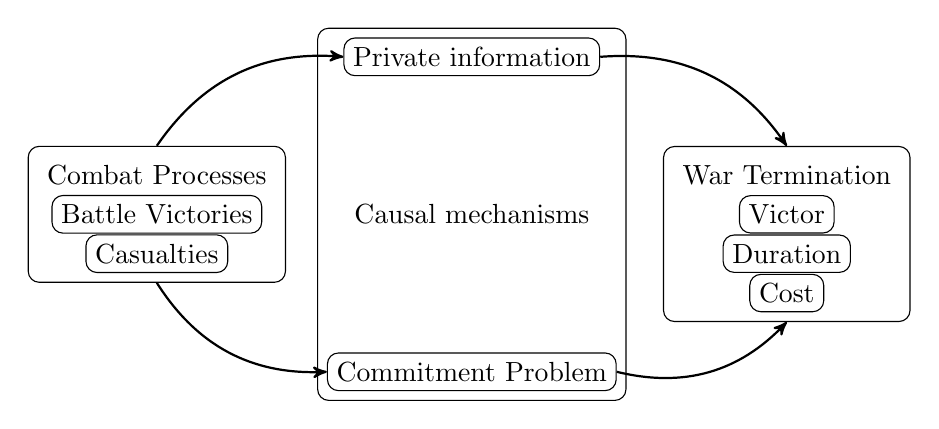
\begin{tikzpicture}[node distance=1cm, auto, scale=0.9]
  % Combat processes
 \node [] (combattitle) (combattitle) {Combat Processes};
 \node [punkt, below of=combattitle, node distance=0.5cm] (victory) {Battle Victories};
 \node [punkt, below of=victory, node distance=0.5cm] (casualties) {Casualties};
 \node [draw, rounded corners, fit={(combattitle) (victory) (casualties)}] (combat) {};

 % casual mechanisms
 \node [right of=combat, node distance=4cm] (dummy) {Causal mechanisms};
 \node [punkt, above of=dummy, node distance=2cm] (pi) {Private information};
 \node [punkt, below of=dummy, node distance=2cm] (cp) {Commitment
   Problem};
 \node [draw, rectouter, fit={(dummy) (pi) (cp)}] (causal) {};

 % war termination
 \node [punkt, right of=dummy, node distance=4cm] (wvictor)
 {Victor};
 \node [punkt, below of=wvictor, node distance=0.5cm] (wduration)
 {Duration};
 \node [punkt, below of=wduration, node distance=0.5cm] (wcost)
 {Cost};
 \node [above of=wvictor, node distance=0.5cm] (wterm)  {War Termination};
 \node[draw, rectouter, fit={(wterm) (wvictor) (wduration) (wcost)}] (end) {};

 % paths
 \draw [pil] (combat.north) to [bend left] (pi.west);
 \draw[pil] (combat.south) to [bend right] (cp.west);
 \draw[pil] (pi.east) to [bend left] (end.north);
 \draw[pil] (cp.east) to [bend right] (end.south);
\end{tikzpicture}
  \caption{Combat and War Termination}
  \label{bonds_battles:fig:combat-causal-diagram}
\end{figure}

Formal models can be classified by the casual mechanism by which combat influences war termination and by the means of combat. %
The formal models differ not only alter the mechanism in which they are interested (private information or commitment), but also the role of battles in the war, and the nature of the combat process: whether battles are important primarily because they impose costs (resolve), or because they can create war victory (probability of victory). %
Battle victory can bring total victory or collapse in war, either suddenly \parencites{Powell2004}{Wagner2000}{LeventogluSlantchev2007}, or over time \parencites{Slantchev2003}{SmithStam2004}.
Battles also impose costs \parencites{FilsonWerner2002}{Powell2004}{LeventogluSlantchev2007}. %

The second approach, which is adopted in this paper, is to focus on which observable features of battles effect war termination, regardless of whether those effects occur through the private information or commitment problem channels. This appears in formal models as well. %
Bargaining is conditioned on the military combat process of war, and what would happen if that process continues to completion.

This bargaining is conditional on the state of that process or
expectations about the future state of that combat process.
\textcite[135]{Wagner2000} writes,
\begin{quotation}
  while states that are fighting may not actually try to disarm each
  other, they must bear in mind the fact that they could, and absolute
  way, even though it never occurs, must be the ``measure of all their
  hopes and fears.''
\end{quotation}

This approach is closer to earlier pre-bargaining empirical work on war (initiation) except in that it involves within war variables. %
The reason is that identifying the channel through which war events influences the end of war is empirically quite difficult. %
For almost any observable data of war outcomes, it both alters the actual state of the war and the beliefs of the participants about the combat process in which they are involved. %
And as of yet, there are no general results with empirical implications that differentiate between

There are a couple ways in which this effects might be identified. %
First, if the beliefs of the participants were observed, then the effects of war events on the beliefs of the participants could be measured. %
One problem with this is that it is hard to observe the beliefs of the participants, even if diaries or reports are available, it is not clear whether these are accurate indicators of those beliefs. %
Another problem, is that it is insufficient to simply observe changes in the beliefs of one participant over time, as in \textcite{Reiter2009}. %
The causal mechanism in informational theories of war is the \textit{convergence} of beliefs of the belligerents to a common distribution. %
This requires knowing the beliefs of both sides, both the mean and variance of those beliefs, or at the very least, the variance of prior distribution based on public information. %
By using documentary data, \textcite{Goemans2000} and \textcite{Reiter2009} are able to do this.
Second, identification would have to rely on a much more detailed model of military combat and war than exists now.
However, this would require more work along the lines of \textcite{Biddle2004}, which focus on generating models of military combat correct, even if these models are not directly tied to political variables.

This is not to abandon the bargaining theory of war or to claim it is useless.
It is to argue that the current incarnation of the theory require a deeper understanding of the specifics of the bargaining process and the combat process in order to develop models with empirical implications.
And that understanding of the specifics of those processes does not spring like Athena fully formed from the head of Zeus, but will come from the study of wars, and developing stylized facts and empirical patterns which will serve as the assumptions of models.

Nor are the extant formal models of war particularly useful, or designed for empirical testing. %
The models are written at a high level, and the causal mechanisms are generally unobservable variables. %
They establish what sorts of explanations of war are complete, and what sorts of explanations and models are not (anarchy, balance of power, offense-defensive balance).
This is nontrivial, as \textcite{Fearon1995} ruled out a number of classes of explanations as having insufficient argument, and also established that war can explained within a rational framework, without relying on ex post irrationality or misperceptions of the participants.
However, the parameters is the models have only a tenuous mapping to the real world. %
The comparative statics in the models are generally determined by specific features of the bargaining framework and it is unclear whether these are general conditions. %
For example, there are claims that wars of information must be short based on \textcite{Slantchev2003} because in that model war can only last 3 rounds. %
However, that result is a direct result of the assumption that there are three types; increase the number of types (or the variance in the power of those types) and the duration of the war increases. %
\textcite{Powell2004} empirical implication is that wars of uncertainty about resolve are shorter than those of uncertainty about fighting. %
That result follows from the feature that costs are incurred between battles; but if costs can be incurred without fighting, and that is enough to allow for the resolution of combat, then why fight at all?

Much of the discussion of models of war has discussed whether war is bargaining or commitment.
However, also important is the nature of the combat process that underlies the bargaining model. %
The difficulty is that these processes may be extremely heterogeneous, across time and space \parencite{Reiter2003}.
But these are not reasons to ignore the processes, but patterns to be understood and explained. %
For while war may look different and be fought differently in time and
space, there must be similarities in it, or we would not call of those events ``war''. %
Moreover, understanding the different forms of the combat process is important to understanding how information and commitment problems are resolved through conflict. %
Better identifying the combat processes present in wars may provide different implications of those models, and thus make it easier to
distinguish when or if they are present.%
\footnote{%
  For example, \textcite{Walter2009} conjectures that insurgency is slower to reveal information than other forms of war. %
  Rigorously evaluating theories in this manner would require better theories of the actual military rationale between insurgency versus conventional war, the characteristics of each, and when belligerents choose to use each.
} %



\section{Why The American Civil War?}
\label{bonds_battles:sec:why-american-civil}

The American Civil War is a war with plentiful, and high quality battle-level data, and in which there are financial assets which proxy expected war outcomes well.
In terms of its battle data, the American Civil War is one of the best documented wars, so quality battle-level is available.%
\footnote{%
  For example, \textit{The Official Records of the Union and  Confederate Armies} \parencites{US1901}, published between 1880 and 1901, consists of 128 books in 70 volumes totaling 139 thousand pages.
  
} %
I discuss why financial assets issued by the belligerents of the American Civil War may be particularly useful for understanding war in section \ref{bonds_battles:sec:why-prices-study}.

Like any case, its generalizability is limited by its similarity to other observations. 
But despite its age, the American Civil War is not dissimilar to contemporary civil wars.
First, the American Civil War is, if not the first modern war, one of the wars during the transition to modern warfare.
This war introduced several of the technologies which later came to prominence in World War I and later wars: rifled artillery, telegraph, machine guns, barbed wire, ironclad warships, and submarines \parencites[89][]{Fuller1956a}[760]{Weiss1966}.
Second, the American Civil War was primarily a conventional war.
This places it in the plurality of post-Cold War civil wars, which are more often conventional wars than insurgencies \parencite[423]{kalyvas2010inter}.%
Finally, by the Civil War was industrializing and the purchasing power parity adjusted GDP per capita of the U.S. and Confederate States in 1860 would classify them them as lower-middle income countries today.%
\footnote{%
  The GDP per capita of the US in 1860 was \$2,241 in 1990 GK international dollars. %
  In 2010, Cambodia had a GDP per capita of \$2,450, Pakistan \$2,494, and Ghana \$1,922 \parencite{BoltZanden2013}. %
  The southern states were poorer than the northern states, with a per capita consumption of about 70 percent of the overall U.S. level \parencite[324]{GoldinLewis1975}.
  The GDP per capita of the pre-war Confederacy is similar to that of Angola, Iraq and Senegal in 2010.%
  The estimated GDP per capita of the southern states in 1860 at 70\% that of the northern states was \$1,568. %
  In 2010, the following countries had approximately the same real GDP per capita: Angola \$1,600, Iraq \$1,610, and Senegal \$1,507 \parencite{BoltZanden2013}. %
}

The American Civil War is also an interesting case for study in its own right.
Its importance to American history is obvious, and need not be stated.%
\footnote{See \textcite{McPherson2003} among too many to list.}
But, given the voluminous literature on the subject, it is surprisingly understudied in at least two regards. %
First, the international relations literature has largely ignored this conflict.
While the inter-state war literature considers it a civil war, and the civil war literature focuses on the post-1945 era \parencites[140-141]{Reiter2009}[2]{Poast2012}. %
Exceptions to this are \textcite{Reiter2009} and \textcite{Poast2012}.
Second, almost none of the existing work on the American Civil War conflict, including the few examples in international relations, use quantitative methodologies. %
\footnote{\textcite{Weiss1966} for an example from operations research.}
In applying international relations theory and quantitative methods to the study of this war, this work contributes a droplet to the ocean that is the literature on the American Civil War.


\section{U.S. Government Bond Yield Data}
\label{bonds_battles:sec:why-prices-study}



\subsection{The Fives of 1874}
\label{bonds_battles:sec:5s-1874}

I will use the yields of long-run U.S. government bonds as a measure of the expected outcome of the American Civil War.
While the yields of bonds of the U.S. government are almost certain to have been primarily driven by expectations of the war, they could plausibly be influenced by both expectations of U.S. victory and expectations of the cost of the war.
However, it is likely that the cost and duration of the war is the more important of those factors.
However, using the yield of U.S. government bonds is difficult since while the U.S. issued a large amount of debt during the American Civil War, the U.S. issued relatively little debt in the ante-bellum period.%
\footnote{
  After paying off the debt issued during the War of 1812, the U.S. government had no outstanding debt between 1835 and 1842 \parencite[297]{HomerSylla2005}.
  The debt as a percentage of GDP rose from 1.9 percent in 1860, before the war, to 31.4 percent in 1866, its peak just after the war \parencites{CBO2012}{CBO2012a}.
}
In this paper, I use the the yields of the U.S. 5's of 1874, because it is the only government bond that was both issued prior to the war and quoted throughout the war, meaning that it is the only complete time series from a single asset that spans the war.

The 5's of 1874 were a coupon bond issued under the authorization of the Act of June 14, 1858 to pay for a budget shortfall due to the Panic of 1857, a financial panic and recession.%
\footnote{
  See \textcites[p. 76]{Bayley1882}[78--79]{DeKnight1900}[42-43]{Treasury1863}[300-301, 305]{HomerSylla2005}
}
As their name suggests, the 5's of 1874 were a coupon bond that paid 5 percent semi-annually on January and July, and were redeemable in 1874, meaning it had a maturity of 13--9 years during the period considered here.
Like most U.S. government bonds, the 5's of 1874 paid interest and principal in specie (gold dollars), even after the U.S. Treasury ceased the redemption Greenbacks (U.S. non-interest bearing notes used as currency issued during the war) in gold.
The U.S. currency floated against the gold dollar until the resumption of convertibility on January 1st, 1879 \parencites{Dewey1918}{WillardGuinnaneEtAl1996}.
For this analysis the prices of the bonds will be converted to gold dollars at the current exchange, and the yields of the bonds calculated with the cash flows converted to gold dollars accounting for the current exchange rate and the expected depreciation of the gold dollar.%
\footnote{
  Since the price of bonds was quoted in currency but it paid interest and principal in currency, calculating the yields is difficult since they also incorporated beliefs about the future prices of gold dollars \parencites[Appendix A]{Macaulay1938}{Roll1972}{Calomiris1988}[302-303]{HomerSylla2005}.
  Most bonds, including the 5's of 1874, were priced in U.S. currency but paid specie and often principal in gold dollars.
  This paper accounts for this using a simple method to calculate the future price path of the dollar; it assumes that currency with appreciate at the risk free interest rate of 5 percent until it reaches parity with a gold dollar.
  This follows from an assumption that the risk free rate is constant over the period, and the gold dollar is priced as a risk-free zero-coupon bond with an unknown redemption date \cite{McCandless1996}.
  \textcite{Roll1972} and \textcite{Calomiris1988} estimate the expected depreciation of gold dollars in Greenbacks using differentials in bonds, however those methods cannot be applied to the period considered here.
}
As will be shown, the price and yields calculated in terms of gold dollars fluctuated dramatically throughout the war.
Yet, the price and yield in terms of currency (after January 1, 1862 when the Greenback floated against the gold dollar, were mostly stable.%
\footnote{See \textcite{Roll1972} for an analysis of this phenomena.}
This suggests that investors were less worried about a complete default on payments of the bonds than that the government would redeem interest or principal payments in depreciated currency rather than in specie.

Figures \ref{bonds_battles:fig:fives1874_price} and \ref{bonds_battles:fig:fives1874_yield} plot the price in gold dollars and the yield to maturity of the 5's of 1874.
Prior to mid-1860, the yield of the Fives was low with little variation, fluctuating between 4.5 and 5 percent.%
\footnote{
  This is actually below was generally considered risk-free rate in the U.S. for that period, 5 percent, which \textcite[29]{Elder1863} calls the ``natural rate of interest on [government] Loans''.
  During this period British 3 percent consols had a yield of between of 3.10 and 3.28 \parencite[193]{HomerSylla2005}.
}
After Lincoln's election in November 1860,  the interest rate rose to 6 percent.
After the initiation of the war with the Battle of Sumter (April 12--14, 1861), the yield rose to 8.2 percent.
During the war, between April 1861 and April 1865, the yield fluctuated between 5.2 and 14.7 percent, reaching its peak on July 30, 1864.
After the end of conflict in April 1865, the interest rate returned to stability at 6.5 percent, a rate higher than its pre-war level.

Data on the prices of the 5's of 1874 come from tables in the two leading monthly financial magazines of the era, the \textit{Bankers' Magazine and Statistical Register} and the \textit{The Merchants' Magazine and Commercial Chronicle} \parencites[186]{Mitchell1903}.
In both sources, the quoted prices were for the New York market, and prices were in currency.
I converted Greenbacks to gold dollars using the current exchange rate in New York, using the data of \textcite{Mitchell1908}.%
\footnote{
  Available in digital form at \url{http://eh.net/wp-content/uploads/2013/11/greenback.txt} from \textcite{WillardGuinnaneEtAl1996}.
  I made some corrections to it where there were incorrect transcriptions from the original source.
}
Both sources quote the bonds at irregular, but approximately weekly frequencies: \textit{Bankers' Magazine} (3--15 days, median of 10 days), \textit{Merchants' Magazine} (4--23 days, wit a median of 7 days).
For the analysis, the quotes of these two series are combined into a single series.

I collected and provide the raw financial data used in this work, as well as additional financial and economic from the American Civil War period in the American Civil War Era Financial Data Collection (ACWFD) \parencite{Arnold2015a}.%
\footnote{Also available at The dataset is at \url{http://github.com/jrnold/civil_war_era_findata}.}
This data collection contains bond prices and exchange rates published in the \textit{Bankers' Magazine} and \textit{Merchants' Magazine}, bid-level auction data for U.S. government bond auctions, and miscellaneous financial and economic data for this period from a variety of primary and secondary sources.

The 5's of 1874 were one of several bonds issued by the U.S. government during this period, but it has several advantages over other bond yield series.
The 5's of 1874 was the only coupon bond regularly quoted in the sources considered here for the entire war, April 1861 to May 1865.
Only one other bond was widely traded at the start of the war, the 6's of 1848--1868.
However, \textit{Bankers' Magazine} stops quoting the 6's of 1868 in September 1861.
Another bond, the  6's of 1861--1881 were issued under acts in February and July 1861, but they are not regularly quoted in the \textit{Bankers' Magazine} until September 1861.
The U.S. issued several other bonds of various durations and coupon rates throughout the war, but they provide even shorter time series.
Additionally, in most cases these loans had relatively exotic features, such as an option to exchange for another bond series or being callable by the government, which make it difficult to calculate the yields for them.
\footnote{
  The 5-20's and 10-40's were bonds callable by the government after 5 (10) years and redeemable in 20 (40) years.
  The 7-30's were bonds that had coupon rates of 7.30 percent (2 cents per day), were redeemable in 3 years, but included the option to be exchanged for either the 6's of 1881 or 5-20's.
  See \textcites{Bayley1882}{DeKnight1900}[297--309]{HomerSylla2005} for overviews of U.S. debt issues during this period.
}
Using the 5's of 1874 relative to other bonds should not make a substantive difference, since as Figure \ref{bonds_battles:fig:fives1874_union} shows, the yield to maturity of the 5's of 1874 is similar to the yields of all the other bonds issued by the U.S. government.
\textcites{WillardGuinnaneEtAl1996}{McCandless1996}{SmithSmith1997} use the exchange rate between Greenbacks and gold dollars in their analyses.
However, since the U.S. did not issue currency until after the start of the war, and did not suspend the redemption of that currency for gold until January 1, 1862, any analysis using only Greenback prices cannot cover the first eight months of the war, April--December 1861.
This is the period which should have the highest informational content in an informational theory of war, and includes battles such as the First Battle of Bull Run, and the Battle of Wilson's Creek.%
\footnote{\textcite{Poast2012} argues that the First Battle of Bull Run was pivotal in avoiding British recognition of the Confederate States.}
However, as with the 5's of 1874 versus other bonds,  Figure \ref{bonds_battles:fig:fives1874_greenbacks} shows that the prices of the 5's of 1874 in gold dollars is similar in both level and trend as the the price of Greenbacks in gold dollars, so the choice is unlikely to change the results.

The American Civil War is an ideal case in which to use prices to infer expectations of war termination for three reasons.
First, The war was of such severity that the nearly the entire budget of the U.S. government was war-related military spending, and thus fiscal expectations corresponded to military spending expectations. % 
For the U.S., the War and Navy Departments accounted for 76 percent (in 1862) to 61 percent (in 1865) of the expenditures.
The fraction of the budget spent directly on the military by the Union fell over the course the war as the fraction spent on paying the principal and interest on its debt, increased from 20 (1862) to 36 (1865) percent of the budget.
But, the overwhelming the majority of that debt had been issued to fund the war \parencites{Treasury1861a}{Treasury1861b}{Treasury1862}{Treasury1863}{Treasury1864}{Treasury1865}.
As \textcite[][668]{McCandless1996} states, ``[d]uring the war, the single most important indicator of future government expenditures is the process of the war itself.''
% INSERT FIGURE OF THE BUDGET

Second, there is extensive economic history literature establishing that war events are the single best determinant of bond and currency prices during the American Civil War:
\parencites{Mitchell1903}{Mitchell1908}{Calomiris1988}{WillardGuinnaneEtAl1996}{McCandless1996}{SmithSmith1997}, graybacks \parencites{Schwab1901}{Weidenmier2002}, southern prices
\parencite{BurdekinLangdana1993}, Confederate bonds \parencites{DavisPecquet1990}{BrownBurdekin2000}{OosterlinckWeidenmier2007}, and Union bonds \parencite{Roll1972}.%
\footnote{One notable exception is \textcite{BurdekinWeidenmier2001}, which shows that the prices of graybacks in Richmond and Houston diverged due to differential application of monetary reform in late 1864.}
%These are largely interested in showing that the markets efficiently responded to new information in the war; this paper is inverting that, and starting with the assumption that the markets are efficiently processing new information to understand imporant

Third, statements by and the actions of contemporary investors indicated the importance that war events had on the prices. %
Members of the government, military, and reporters all engaged in investment speculation based on their knowledge of war events \parencites[5-7]{Cornwallis1879}{Mitchell1903}[][1004]{WillardGuinnaneEtAl1996}.
Investment firms even had their own correspondents stationed in cities close to the war fronts to relay the latest news \parencites[5-7]{Cornwallis1879}. %
Finally, magazines and newspapers often cited war events as the cause of recent price movements. %
For example, the issue of \textit{Bankers' Magazine} after Gettysburg and Vicksburg (Jul 23, 1863), cites these battles as the cause of the recent changes in market prices,
\begin{quote}
  The month of July has been a very active one with numerous fluctuations, almost daily, in the market values of gold, with unusual changes in the current values of stocks. %
  The advices as to the war movements are of a most satisfactory kind, leading to a fall in gold from 146 1/2 at the close of June, to 123 1/2, the 20th inst., at which dates the public had learned the  capitulation of Vicksburgh and of Port Hudson, the defeat of Lee in  Maryland and Pennsylvania, and of successful results at other points  for the Union forces. %
\parencite[159]{BankersMagazine1864}
\end{quote}



\subsection{U.S. Government Interest Rates are Primarily a Function of the Expected Cost of the War}
\label{bonds_battles:sec:u.s.-governm-inter}

Since the cash flows of U.S. government bonds are not directly related to a war outcome, in order to treat those yields as an expectation of a war outcome, I need to, first, establish which war outcomes can influence future cash flows, and, second, establish that expectations about war outcomes are the primary factor influencing the yield.
The U.S. government bond yields are plausibly related to both expectations about whether the U.S. would win the war, as well as the cost of the war to the U.S. government.
These two expectations have possibly cross-cutting implications on bond yields, with a increased probability of U.S.\ victory positive (lower yields), but an increased cost negative (higher yields).
Unfortunately, it is not possible to separate these effects using only U.S. government bond yield data.
However, it is likely that U.S.\ government bond yields mostly responded to expectations about the cost of the war, and thus, can be considered a proxy for the expected cost of the war to the U.S.

The riskiness of U.S. government bonds depended on expectations about the cost of the war to the U.S. since the war was funded primarily through debt.
Thus, expectations of a longer or more vigorously fought war almost directly imply and increase in government debt.
The U.S. primarily paid for the war using the debt. 
The proportions of the U.S. government revenues for each source of funding as follows: taxes 72--89\% from loans, 11--25\% from taxes, and 0--4\% from miscellaneous sources (tariffs, land sales).
In its analysis of the future fiscal situation, the 1863 \textit{Annual Report of the Treasury} notes that taxes and other revenue sources were covering the non-war expenses and debt payments in its budget, but new debt was being issued to pay for the military expenditures needed to wage the war \parencite[10-13]{Treasury1863}.
\footnote{See also \textcite[][14]{Godfrey1976}.}
The budgetary effect of the war is clear from  comparing forecasts of the U.S. budget for the 1866 fiscal year made before and after the war had ended.
In \textit{The Annual Report of the  Treasury} issued on December 6, 1864, the forecast deficit for FY 1866, assuming the war continued, was \$470 million, with \$1,168 million in expenditures \parencite[13]{Treasury1864}.
In the following year's \textit{Annual Report} issued in December, 1865, the first after the conclusion of the war, the Treasury estimated a surplus of \$112 million, with expenditures of only \$396 million dollars \parencite{Treasury1865}.
This forecast was close to what would be the actual surplus of \$132 million \parencite[2]{Treasury1866}.
Thus, both expectations of the government military expenditures and the length of the war should have had a direct impacts on investors' expectations of the eventual debt level of the U.S. government.
Since increased debt would increase the possibility of default, it would make the bonds riskier, and the yields higher.

The future resources of the U.S. to pay off that debt also depended on the result of the war, namely, whether the seceding states would be reincorporated into the U.S. and potentially help pay for the costs incurred in the war.
The size and wealth of the seceding Southern states was non-trivial, but still much smaller than those of the Union states.
In 1860, the states that would make up the Confederacy accounted for 29 percent of the overall U.S. population,%
\footnote{
  Southern states included VA, TN, GA, NC, AL, MS, LA, SC, TX, AR, FL \textcite[5]{Eicher2001}.
  Wealth is used instead of 
}
and 25 percent of the total wealth.%
\footnote{
  \textcite[12]{Elder1865}. Wealth is defined as the value personal property excluding slaves, which was asked on the 1860 Census.
  It may be a better measure of how contemporaries would have viewed the value of the South than GDP because GDP had not yet been invented.
  The closest contemporaries had to GDP was an approximation that the value of yearly production was about 25-27 percent of total wealth \parencites[7]{Elder1865}[24]{Treasury1865}.
}
% TODO: What was the Confederacy GDP?

Some statements by government officials and market participants suggest that they are more concerned with the cost and duration of the war than with the the reincorporation of the seceding states.
William Elder, a leading economist of the era, in an 1863 analysis of the ability of the U.S. to repay its debt stated ``The Rebellion leaves our capital in real and personal property just where it was before the secession. \dots{} So far now this is only a loss of that which we have not had, and at best or worst, a very small one in any time of need'' \parencite[19]{Elder1863}.%
\footnote{
  However, \textcite{Elder1863} does emphasize the importance of the resources of the Western territories, which perhaps strengthens the argument of  \textcite{Weingast1998} that he U.S. was concerned that Southern states seceding could lead to Western states seceding.
}
The \textit{Annual Report of the Treasury Department} in 1863 highlighted this relationship between cost of the war and the interest rate it paid on its bonds:
\begin{quote}
It will not escape observation that the average [interest] rate is now increasing, and it is obvious that it must continue to increase with the increase of the proportion of the interest-bearing to the non-interest-bearing debt. 
And as the amount of the latter, consisting of United States notes and fractional currency, cannot be materially augmented without evil consequences of the most serious character, the rate of interest must increase with the debt, and approach continually the highest average.
That must be greater or less in proportion to the duration and cost of the war. \parencite[13]{Treasury1863}
\end{quote}

The striking difference in the trend of the prices of U.S. bonds and that of the Confederate currency (Graybacks) in Figure \ref{bonds_battles:fig:fives1874_compared} is evidence that U.S. bond yields were not driven by expectations of U.S. victory, and, by elimination, likely represent the cost of war to the U.S.
The price of the Confederate currency decreases almost monotonically over the entire course of the war.
Although the price of Graybacks is partially determined by the money supply \parencite{BurdekinWeidenmier2001}, the price of Confederate bonds issued in Amsterdam and payable in gold followed a similar nearly monotonically decreasing trend mid-1863 onward \parencite{HaberMitchenerOosterlinckEtAl2015}.
The prices of the Confederate assets were likely primarily determined by whether the U.S. would win the war and repudiate their debt \parencite{HaberMitchenerOosterlinckEtAl2015}.
If the U.S. bonds reflected the probability of U.S. victory, then the expected trend of its prices (yields) would increase (decrease) immediately after the start of the war, and almost monotonically increase (decrease) throughout the war, or at least from mid-1863 onward.
However, Figure \ref{bonds_battles:fig:fives1874_yield} shows that while the yields of U.S. government bonds fluctuates early in the war, they do not decrease over the course of the war.
Instead, they spike in mid-1864 at a point which U.S. victory should have been highly probable if not almost certain. 
This suggests that U.S. government interest rates are not primarily reflecting expectations of the war result, and are, instead, reflecting some other factor, which is likely the cost of the war.

Finally, the financial benefit of victory and the costs and duration of war are inversely related.
The longer and more destructive the war, the less the ability of the Southern states to provide for the repayment of the debt incurred by the U.S. in fighting the war.
In fact, immediately after the war, the U.S. government attempted to collect direct taxes from the Southern states, but it soon suspended the collection of the direct taxes after it became clear that the Southern states could not pay them.
Treasury Secretary Hugh McCullough justified this suspension by noting that the inhabitants of the Southern states ``had been subject to heavy taxation by the government which was attempted to be established in opposition to that of the United States, and had been greatly exhausted by the ravages of war.'' \parencite[29]{Treasury1865}.
In analyses of the repayment of debt after the war by the Treasury Department and others \parencites{Elder1865}{Treasury1865}{Walker1865a}, the wealth of the Confederate states was assumed to remain constant between 1860 and 1870 due to the destruction of the war, and that they would not be able to contribute to the repayment of the debt until after 1870.

% todo: longer war reduced the pie. Confederacy in worse shape to repay the debt. E.g. ability to extract a direct tax.

While the precise meaning of the bond yields in terms of a war outcome is unclear, it is clear that the bond yields reflect a war outcome and are being driven almost completely by expectations of the war.
As noted earlier in this section, military expenses accounted for the overwhelming majority of U.S. government expenditures between 1861 and 1865, so there are no other budgetary concerns that could plausibly affecting investor's expectations.
The importance of the war can also be seen by comparing the level and variance of U.S. government bond yields during the war with the preceding period.
During 1856--1860 yields on U.S. government bonds were stable at below 5 percent.
At the height of the the Panic of 1857, the yield of U.S. government bonds, the 6's of 1868, only reached 5.1 percent.%
\footnote{Source: Data from the \textit{Bankers' Magazine} and the author's calculations. Also see \textcite{HomerSylla2005}.}
Since a major financial crisis had little effect on bond yields prior to the war, there are certainly no non-war omitted factors affecting the yields.
This is not to say that the battles in the war are the only factor affecting the bond yields.
Government policies, elections, and other events could and almost certainly had some affect on bond yields.
But all of these other events were affecting the government bond yields through their effects on expectations of investors' of the eventual outcome of the war.

In summary, the U.S. government bond yields reflected some combination of expectations about the cost, duration and the victor of the war, weighted by how each of these would affect the ability of the U.S. government to repay its debts.
However, it is more likely that these yields are largely reflecting expectations about the cost and duration of the war.

\begin{figure}[!]
  \centering
  \begin{subfigure}[b]{\linewidth}
   \includegraphics{../bonds_and_battles//paper/figure/fives1874_price-1}
  \caption{Price in gold dollars. Par value is \$100.}
  \label{bonds_battles:fig:fives1874_price}
\end{subfigure}
\begin{subfigure}[b]{\linewidth}
   \includegraphics{../bonds_and_battles//paper/figure/fives1874_yield-1}
  \caption{Yield to maturity.}
  \label{bonds_battles:fig:fives1874_yield}
\end{subfigure}
\caption[Price and yield of the 5's of 1874, 1858-1865]{Price and yield of the 5's of 1874 from its issue in 1858 until the end of the Civil War in 1865.
The yield is steady at near 5 percent until the election of Lincoln and the secession of the Southern States in late 1860-early 1861.
During the American Civil War, the yields are variable, spiking in the middle of 1864.
 }
\label{bonds_battles:fig:fives1874_yield_price}
\end{figure}

\begin{figure}[!]
  \begin{subfigure}[b]{0.45\linewidth}
    \includegraphics{../bonds_and_battles//paper/figure/fives1874_greenback_price-1}
  \caption{Price in gold dollars for the 5's of 1874 compared to the price of Greenbacks, 1862-1865.}
  \label{bonds_battles:fig:fives1874_greenbacks}
\end{subfigure}%
\hspace{0.1\linewidth}%
\begin{subfigure}[b]{0.45\linewidth}
    \includegraphics{../bonds_and_battles//paper/figure/fives1874_union-1}
    \caption{Yield to maturity of the 5's of 1874 compared with other U.S. bonds.}
  \label{bonds_battles:fig:fives1874_union}
\end{subfigure}

%% \begin{subfigure}[b]{0.45\linewidth}
%%   \centering
%%   \includegraphics{file.path(fig_path, "fives1874_north-1")}
%% \caption{Yield to maturity of the 5's of 1874 compared with bonds issued by Northern states.}
%% \label{bonds_battles:fig:fives1874_north}
%% \end{subfigure}%
%% \hspace{0.1\linewidth}%
%% \begin{subfigure}[b]{0.45\linewidth}
%%   \includegraphics{file.path(fig_path, "fives1874_south-1")}
%% \caption{Yield to maturity of the 5's of 1874 compared with bonds issued by Southern and border states.}
%% \label{bonds_battles:fig:fives1874_south}
%% \end{subfigure}

\begin{subfigure}[b]{0.45\linewidth}
  \includegraphics{../bonds_and_battles//paper/figure/fives1874_graybacks-1}
\caption{Price in gold dollars of the 5's of 1874 compared with \$100 Graybacks (Confederate currency).}
\label{bonds_battles:fig:fives1874_grayback}
\end{subfigure}
\caption[The 5's of 1874 compared with other government and states issued bonds and currency.]{The 5's of 1874 compared with other government and states issued bonds and currency.
  The 5's of 1874 follow a similar pattern as that of other U.S. bonds and those issued by Northern states.
  They diverge and have a different pattern than the Confederate currency and bonds issued by Southern states.
}
\label{bonds_battles:fig:fives1874_compared}
\end{figure}

% TODO: this needs qualitative overview of the 


\section{Battle Data}
\label{bonds_battles:sec:battle-data}

A theoretical and practical issue in the empirical study of war is how to operationalize military combat within wars.%
\footnote{
  See the discussions in \textcites{ReiterStam1998}{BiddleLong2004}{Reiter2003}{GrauerHorowitz2012}{Weisiger2015}.
} 
There are two major issues in the operationalization of military combat.
The first is ``what the unit of observation?''.
Some work uses events, such as battles or campaigns, as the unit of observation \parencites{ReiterStam1998}{ReiterStam2002}{Ramsay2008}{PilsterBoehmelt2011a}{GrauerHorowitz2012}, while other work uses time-period aggregated values, \eg{} monthly casualties \textcite{Weisiger2015}.
The second is ``how to measure military success?''.
Some work uses the categorical measures of victory or defeat in battle \parencites{ReiterStam1998}{ReiterStam2002}{GrauerHorowitz2012}, while other work uses casualty based measures, such as the loss-exchange ratio  \parencites{Biddle2004}{BiddleLong2004}{PilsterBoehmelt2011a}.
In this work, quantify military combat in the American Civil War by focusing my analysis on a set of ``militarily significant'' battles, and define success in combat by a categorical coding of their result: Union or Confederate victory.
An advantage of this method is that it allows me to effects individual battles without fewer assumptions of how features of those battles relate to war outcomes, and as well as the average effect of Union and Confederate battle victories.

The battles used in the analysis are listed in Table \ref{bonds_battles:tab:battles}.
This is the set of the battles which the National Park Service's Civil War Sites Advisory Commission (CWSAC) defined as the most militarily significant in the war, which they defined as ``having a decisive influence on a campaign and a direct impact on the course of the war'' \parencite{CWSAC1993}.
These data come from the 1993 CWSAC report, Civil War Sites Advisory Commission Report on the Nation's Civil War Battlefields \parencites{CWSAC1993}{CWSAC1993b}.
The CWSAC was established in accordance with a 1990 law to preserve Civil War battlefields and was ``asked to identify the nation's historically significant Civil War sites; determine their relative importance; determine their condition; assess threats to their integrity; and recommend alternatives for preserving and interpreting them.'' \parencite{CWSAC1993b}
As part of that process they identified 383 battles, of the over 10,500 military engagements listed in the \textit{Official Records of the American Civil War}, as the ``principal battles'' of the war based on a ``military significance'' criteria. 
As to the comprehensiveness of their list, \parencite{CWSAC1993} states,
\begin{quote}
  These [battle] sites encompass virtually all of the principal land battles that were of special strategic, tactical, or thematic importance to local operations, campaigns, theaters, or to the war as a whole \dots{} 
  The more than 10,500 conflict sites excluded from our inventory were relatively unimportant as individual military actions.
  These conflicts were the venues and actions that implemented the war between and beyond the dramatic major engagements. 
\end{quote}
These principal battles were further classified into four categories of military significance: A (``having a decisive influence on a campaign and a direct impact on the course of the war'') to D (``having a limited influence on the outcome of their campaign or operation but achieving or affecting important local objectives'').
This work will use  42 battles with the ``A'' military significance classification.%
\footnote{
  Three CWSAC class ``A'' battles are omitted from the analysis.
  The Battle of Fort Sumter (SC, April 12--14, 1861) is omitted because it marks the start of the war and the analysis starts after this battle.
  Given the small size of Fort Sumter, no casualties, the effects of the battle can be attributed to marking the start of conflict.
  The Battle of Fort Blakely (AL, April 2--9, 1865) is omitted because news of battle does not reach New York City until after news of the surrender of Gen. Robert E. Lee's forces at Appomattox Court House on Apr 10, 1865.
  The Battle of Five Forks (VA, April 1, 1865) is omitted because I could not find reports of it in the \textit{New York Times}; news of it was overshadowed by Third Battle of Petersburg on April 2nd, which ended the Siege of Petersburg.
}
While this is a subset of the battles, it is still a relatively large number of battles by most war standards and similar in number and composition as the list of battles in other sources: \textcite{Livermore1900} includes 63 battles, \textcite{Bodart1908} includes 50, \textcite{cdb90} includes 49.
Although this is the may be considered a subset of battle of the American Civil War, that is largely due to the completeness of the records and richness of the data on the American Civil War.

\begin{figure}[htpb]
  \centering
  \includegraphics{../bonds_and_battles//paper/figure/fig_major_battles-1}
  \caption{Major battles and their outcomes}
  \label{bonds_battles:fig:major_battles}
\end{figure}

The CWSAC report \parencite{CWSAC1993b} gives each battle a result, which is one of ``Union victory'', ``Confederate victory'', and ``Inconclusive''.
While \textcite{CWSAC1993} does not explicitly describe the methodology used to classify the battle outcomes, the classifications largely agree with other sources \parencites{fox1898regimental}{Livermore1900}{Bodart1908}{cdb90}, several of which are themselves cited as sources in the report.
Two of those sources, \textcite{fox1898regimental} and \textcite{Livermore1900}, provide more description of how they assigning victory.
Generally, the victorious side of a battle is considered to be the side that controls the battlefield at the end of battle.
The data used in this paper includes 29 Union victories, 13 Confederate victories, and two ``Inconclusive'' battles.
For the analysis, the two ``Inconclusive'' battles,  The Wilderness, and Spotsylvania Court House, will be recoded since with only two battles, I cannot estimate an average effect of ``Inconclusive'' battles.
The Wilderness was reclassified as a Union victory, and Spotsylvania Court House as a Confederate victory based on how the results were reported in the news.
Figure \ref{bonds_battles:fig:major_battles} plots the date and outcomes of these battles over time.%
Since these by selecting on the most militarily significant battles, I have already effectively selected those battles with the highest casualties and force sizes, I will not explicitly include casualty or force size related variables in the analysis.

\begin{table}
  \centering
  \input{../bonds_and_battles//paper/tex/tab_major_battles.tex}
  \caption{List of the 42 major battles of the American Civil War included in this analysis.}
  \label{bonds_battles:tab:battles}
\end{table}

The final data that I need in order to estimate the effects of these battles on bond yields are the times at which the New York markets received news about these battles.
This is not the same as the date of the battle, but occurs with some lag.
But in general, New York markets received news about battles surprisingly quickly:
\begin{quote}
Members of both Houses [of Congress], and of all political creeds, resident bankers, the lobby agents, clerks, and secretaries, haunted the War Department for the latest news from the seat of war.
The daily registry of the Gold Room was a quicker messenger of successes or defeats than the tardier telegrams of the Associated Press. A private secretary of a high official, with no capital at all save his position, which gave him authentic information of every shaping of the chess game of war a full twenty hours in advance of the public, simply flashed the words ``sell, buy'' across the wires, and trusted to the honor of his broker for the rest. \parencite[245]{Medbery1870a}\footnote{Originally quoted in \textcite{WillardGuinnaneEtAl1996}.}
\end{quote}
However, there was still a lag between the occurrence of the battle, and when news of the outcome.
More importantly for the analysis, this lag varied with the distance of the battle from New York and Washington, as well as some idiosyncratic circumstances.
For example, the market knew nothing of Sherman's army after he moved north from Savannah until he arrive d  to the sea until he arrived  \textcite[204]{Mitchell1903}.
As a measure of when information of the battle reaches the New York market, I coded when news about a battle was first reported in the \textit{New York Times}.
This was not necessarily one day, for some battles (Chattanooga) which lasted several days of approximately equal intensity, I coded news reaching the market on several days.
However, for sieges which could last many days, \eg{}Vicksburg, Port Hudson, I only coded when news of the end of the siege was reported.
While battles the Eastern theater were reported on the same or next day (Antietam, Gettysburg), news on battles in other theaters may not reach the market for days.
The battle with the longest lag in news was the Battle of Glorietta Pass in New Mexico; it ended on March 28, 1862, but news of the battle did not reach New York city until April 15.
A data driven approach to identifying the timing of this news is important since in a time series analysis, the timing of the events is the primary factor in identifying their effects.
% Illustrative anecdotes: McClellan in Peninsula campaign, Sherman in march to the sea.

In using a small set of battles based on a \textit{ex post} expert assessment of their military importance, it is important to note that this is not selecting on the dependent variable.
In this case, that would be including explanatory variables by selecting periods of times that had large changes in yields.
Instead, i am selecting a set of covariates, \ie{} battles, which are expected to have large effects on the response variable based on prior information.
This is no different than any other regression model, in which only a small set of covariates are selected of all possible variables in the universe, because those covariates are \textit{a priori} expected to plausibly have effect on the response variable.

For this project, I created a public data collection of American Civil War battles, the American Civil War Battle Database (ACWBD) \parencite{Arnold2015b}.%
\footnote{The data and source code of the data collection are available from \url{https://github.com/jrnold/acw_battle_data}.}
The ACWBD combines, cleans, cross-references battle data from multiple primary and secondary sources, including \textcites{Phisterer1883}{Livermore1900}{Bodart1908}{dyer1908_war_rebel}{KennedyConservation1998}{CWSAC1993}{cwsac2012}.
It is the most complete, machine-readable data on American Civil War battles of which I am aware.



\section{Model of War Events on Yields}
\label{bonds_battles:sec:model-war-events}

In this section, I present a model of the U.S. government bond yields as a function of battles.
As noted in Section \ref{bonds_battles:sec:5s-1874}, the yields of 5's of 1874 will be used for the measure of the interest rate.

As seen in Figure \ref{bonds_battles:fig:fives1874_yield}, the variance of the changes in the yields tends to increase with the level. 
To account for that in the model, I will model the logarithm of the yields.
Let $y_{i}$ be the natural logarithm of the yield.
I suppose that the observed log yields are observed with measurement error,%
\footnote{Equation (\ref{bonds_battles:eq:1}) is simplified for presentation. Since two sources are used, and in some cases there are multiple observations, $y_{t}$ is the mean of the observations, and $\tau_{t} = \tau / \sqrt{n_{t}}$ where $n_{t} \in \{1, 2\}$ is the number of observations on that day.}
\begin{align}
  \label{bonds_battles:eq:6}
  y_{t} &= \mu_{t} + \epsilon_{t} & \epsilon_{t} \sim \dnorm{0, \tau^{2}}
\end{align}
The effects of battles and other events are included in the equation which models the latent log-yields.
The first difference of the log yields is a function of a time-varying trend $\alpha_{t}$, and the effects of battles $W_{t} \beta$, and other events $X_{t} \gamma$ 
\begin{align}
  \label{bonds_battles:eq:7}
  \mu_{t} &= \mu_{t - 1} + \alpha_{t} + W_{t} \beta + X_{t} \gamma + \omega_{\mu,t}
\end{align}

The matrix $W$ contains a daily weight term for each battle which is non-zero if the news of the battle ``reached the market'' on that day, and zero otherwise.
Each column of $W$ sums to one, so the $\beta_{b}$ is the total effect of battle $b$,
\begin{align}
  \label{bonds_battles:eq:1}
  \mu_{i} &= \sum_{k = t[i-1] + 1}^{t[i]} \sum_{b \in B} w_{b,k} \beta_{b}
\end{align}
The effect of a battle in a period is the sum of the product of a daily weight term $w_{b,k}$ ($\sum_{t \in 1:T} w_{b,t} = 1$) and its overall effect $\beta_{b}$.
The weight terms are equally weighted for each battle and non-zero on the 1st day(s) in which news of the battle was reported and a lag of XXXX days.
For example, the end of Gettysburg was reported in the news on XXXX, so XXXXX through XXXX (XXXX days later) have a weight of XXXX, and all other days have a weight of 0.

The effects of battles are modeled as coming from two distributions: Union victories, and Confederate victories.
\begin{equation}
  \label{bonds_battles:eq:4}
  \begin{aligned}[t]
  \beta_{b} &\sim
  \begin{cases}
    N(\gamma_{\mathtt{U}}, \zeta^{2}) & \text{if $b$ is a Union victory} \\
    N(\gamma_{\mathtt{C}}, \zeta^{2}) & \text{if $b$ is a Confederate victory}
  \end{cases}
  \end{aligned}
\end{equation}
This model allows for the estimation of the average effect of Union and Confederate victories ($\gamma$) while allowing for the effects to vary between battles and by extension over time.
The distributions share a common scale, $\zeta^{2}$, since there is not enough data to estimate separate scales well.

The error in Equation (\ref{bonds_battles:eq:7}) is modeled as a stochastic volatility process,
\begin{equation*}
  \label{bonds_battles:eq:9}
  \begin{aligned}[t]
    \omega_{\mu,t} & \sim \dnorm(0, \sigma_{\omega, t}) \\
    \log \sigma_{\omega} &\sim \dnorm(\bar{\omega} + \rho_{\omega} \log \sigma_{\omega, t - 1}, \xi)
  \end{aligned}
\end{equation*}
The trend follows an AR(1) process.
This is meant to account for unobserved trends in the conduct of the war that are not picked up by the observed variables.
\begin{align}
  \label{bonds_battles:eq:8}
  \alpha_{t} &\sim \dnorm(\rho_{\alpha} \alpha_{t - 1}, \sigma_{\alpha}^{2})
\end{align}

The posterior distribution of the was sampled with MCMC using the NUTS-HMC algorithm as implemented in Stan.%
\footnote{See \parencites{Stan2015a}.}
Thus far, in this section, I have only discussed battle data but battles not the only relevant events in a war, and this war in particular.
Changes in policy, leadership, foreign policy events, negotiations and other events may all influence expectations about the future of the war.
The first is that it is difficult to coherently choose a set of events.
\textcite{McCandless1996} and \textcite{SmithSmith1997} both include lists of indicator variables for \textit{ad hoc} lists of military, fiscal, and political events in the war.
However, there is no clear rule as to what constitutes major non-battle events in the war, and what does not.
\textcite{SmithSmith1997} includes indicator variables for a list of war, and political and financial news, but these are generated by selecting on the dependent variable, by using events mentioned in \textcite{Mitchell1903} as corresponding to large daily movements in the gold market.%
\footnote{
  An exception to this is funding bills, where their effect can be modeled as a function of how much each bill increases the debt.
  The difficulty of including funding bills is the effect on the market should not occur when the bill is signed, which is easy, but during the negotiations of the bill when information about the possible outcome of the vote is known.
}
The second reason is that non-battlefield events are more likely influenced by battlefield events than vice versa.
For example, the capture of Atlanta is given as a reason why Lincoln won the election of 1864.
The outcomes of battles influence expectations about the entire future course of the war, including non-battle events.
Thus, the effects of the non-battle events on the prices and yields of financial assets is only the surprising part, only the events that are not anticipated given the previous events on the battlefield.
Since I do not include data on non-war events in the war, in the models of Section \ref{bonds_battles:sec:model-war-events} I will account for these events using fat-tailed distributions (Student's $t$) in the error term to allow for the effects of large events, although they are not included explicitly.
In Section \ref{bonds_battles:sec:conclusion}, I propose a more coherent method for identifying war and non-war events.


\footnote{
  Two things are missing from this model that are common in models involving interest rates: inflation and a risk-free interest rate.
  Inflation is not included for several reasons.
  First, while inflation measured in Greenbacks rose during this period, since the price of gold tracked the price of commodities during this period, inflation in terms of gold dollars was low\parencites{Mitchell1903}{Mitchell1908}.
  Second, even if that were not the case, the influence of the war was such that inflation would likely be considered a post-treatment variable that was responding to war events.
  Third, the best measure of inflation, the Warren-Pearson Wholesale Price Index, is only available at the monthly level.
  The risk free interest rate during this period is not used because it is hard to define one during this time \parencites{HomerSylla2005}.
  In later periods, U.S. government bonds would be considered a risk free interest rate.
  But this work uses U.S. government bonds precisely because they are risky with that risk varying with expectations of the war outcome.
  \textcites{Macaulay1938}{HomerSylla2005} consider two other bond indexes as risk free interest rates: railroad bonds and New England municipal and state bonds.
  During this period, railroad bonds were still relatively risky during this period, and had higher yields than U.S. government bonds.
  Municipal bonds, when their yields are calculated in gold dollars, have yields similar to those of U.S. government bonds, and thus were not much less risky.
  Additionally, the only available source of these interest rates, \textcite{Macaulay1938}, provides these interest rates at a monthly (railroad) and quarterly (New England municipals) frequency.
  Other work in 19th century economic history use the interest rate of British consols is used as a risk free interest rate, but that is the 
  This is inappropriate for this analysis because that risk free interest rate was for the London market, and not the New York market.

}

\section{Conclusion and Future Work}
\label{bonds_battles:sec:conclusion}

SUMMARY 


I will conclude with some thoughts on future directions of this research.
There are some issues that I find problematic with the methodology employed in this paper, but which could be addressed by using text data such as newspapers from the period instead of or in addition to \textit{ex post} coded events.
These issues all revolve around identifying what information reaches markets and when. 
Events do not have direct effects on the prices, but are mediated by the signals that the market observes of the events themselves.
These should be related to the actual characteristics of those events, but there will be measurement error.
What is needed are better measures of what the market knew, and when.
This paper handles the what by identifying a set of important battles and their classification as victories or defeats, both of which are determined by historians with the benefit of hindsight.
I could include other factors of the battles --- casualties, attacker, etc. --- but it is not clear how many and how close these measurements were to what the market observed.

The first issue is the lag of events.
  When considering the effect of events on markets, it is not the time of the event \textit{per se} that is important, but the time at which \textit{information} about the event reaches the market.
  This can be handled through modeling --- \eg{}estimating the lag structure, allowing for different different lags around events.
  However, these modeling strategies often implicitly rely on homogeneity of the lag across events to identify the effect.
  It can become difficult when there is heterogeneity in events.
  As noted in Section \ref{bonds_battles:sec:battle-data}, battles Virginia were known the next day, but information from battles in the West would take longer to reach the market.

The second issue is in confounding variables.
  This can be handled by including other variables and dummy variables for events in the analysis.
  But how does one handle the inclusion of these in a principled manner, especially when there are \textit{sui generis} events like the Emancipation Proclamation in the data?

Using contemporary text data from newspaper articles provide a means to address all of these concerns.
The rough sketch of the analysis would be to estimate topics from the text and regress those topics on market movements.
The timing and content of the information reaching the market could be inferred in a data-driven manner from the newspaper texts.
Prior information about important events and characteristics of those events need not be completely thrown away; 
semi-supervised and 
This makes the assumption that the newspaper articles sufficiently reflects the information available to the market, which may seem extreme, but seems less problematic than the issues discussed earlier.
The importance of events relative to other events is identified through their prominence in the newspapers, \eg{}if the front page is about a battle, then it is probably the news that is moving the market, whereas if the frontage is about the passage of a law or the economy, then that is probably the more important news.


%%% Local Variables:
%%% TeX-master: dissertation.tex
%%% End:

%  LocalWords:  Gartzke2007 DafoeKelsey2014a Slantchev2012a 'hide' se
LocalWords:  tex RData barg parencites Peace'' textcite cha financ
LocalWords:  outcome'' result'' GuidolinLaFerrara2010 Lau2006 premia
%  LocalWords:  HaberMitchenerOosterlinckEtAl2015 RhodeStrumpf2004a
%  LocalWords:  WolfersZitzewitz2004 Intrade Tradesports Osama CDB90
%  LocalWords:  LeighWolfersEtAl2003 Slantcheve2012a Hall2004 Uppsala
%  LocalWords:  McCandless1996 ChenSiems2004 SchneiderTroeger2006 pre
%  LocalWords:  WolfersZitzewitz2009 Fearon1995 Reiter2003 Powell2004
%  LocalWords:  FilsonWerner2002 Slantchev2003 SmithStam2004 cdb90
%  LocalWords:  LeventogluSlantchev2007 LangloisLanglois2009 ACLED
%  LocalWords:  WolfordReiterCarrubba2011 belligerents' ESOC US1901
%  LocalWords:  SarkeesWayman2010 BiddleLong2004 Clodfelter2008 5's
%  LocalWords:  CochranLong2014 RaleighLinkeHegreEtAl2010 Reiter2009
%  LocalWords:  Goemans2000 WillardGuinnaneEtAl1996 north2000introd
%  LocalWords:  FreyKucher2000 FreyKucher2000a Cornwallis1879 consols
%  LocalWords:  Mitchell1903 investors' Ramsay2008 Weisiger2015 ACWFD
%  LocalWords:  Keele2015a Wagner2000 Biddle2004 misperceptions OKFN
%  LocalWords:  Walter2009 Mitchell1908 Calomiris1988 SmithSmith1997
%  LocalWords:  Schwab1901 Weidenmier2002 BurdekinLangdana1993 sumter
%  LocalWords:  DavisPecquet1990 BrownBurdekin2000 Roll1972 Weiss1966
%  LocalWords:  OosterlinckWeidenmier2007 generalizability Poast2012
%  LocalWords:  Fuller1956a multimanned kalyvas2010inter Bayley1882
%  LocalWords:  BoltZanden2013 GoldinLewis1975 McPherson2003 maxdate
%  LocalWords:  hacker2011census Livermore1900 DeKnight1900 Dewey1918
%  LocalWords:  Treasury1863 HomerSylla2005 fives1874 Elder1863 6's
%  LocalWords:  Bankers' Merchants' Macaulay1938 Arnold2015a 20's HMC
%  LocalWords:  40's 30's Ball1991 Treasury1861a Treasury1861b uring
%  LocalWords:  Treasury1862 Treasury1864 Treasury1865 graybacks nrow
%  LocalWords:  BurdekinWeidenmier2001 Vicksburgh BankersMagazine1864
%  LocalWords:  COFEDERACY Godfrey1976 Treasury1866 ReiterStam1998
%  LocalWords:  ReiterStam2002 PilsterBoehmelt2011a CWSAC CWSAC1993
%  LocalWords:  GrauerHorowitz2012 CWSAC1993b Blakely Bodart1908 CWSA
%  LocalWords:  fox1898regimental Spotsylvania Medbery1870a Glorietta
%  LocalWords:  Arnold2015b Phisterer1883 dyer1908 cwsac2012 XXXX sui
%  LocalWords:  KennedyConservation1998 XXXXX MCMC Stan2015a generis
%  LocalWords:  bellum CBO2012 CBO2012a 5's 6's 20's 40's 30's bodart
%%  LocalWords:  Eicher2001 Elder1865 Weingast1998 Walker1865a
%%  LocalWords:  livermore
